\chapter{BLI Modeling Phase}
	In the previous chapter, the overall BLIPSS methodology was developed and hypotheses 1 and 2 were made based on observations from past literature and additional theoretical analysis.  This chapter will demonstrate the BLI modeling phase, as outlined in Chapter 3, for a canonical design problem involving a hybrid wing body vehicle with boundary layer ingesting turbofan engines.  The chapter will proceed according to the outline of the BLI modeling phase and the BLI component modeling process defined in Chapter 3.  Furthermore, experiments intended to validate hypotheses 1 and 2 will be defined and conducted in order to justify the need for each of the components of the method and to determine which physical effects are relatively important for this canonical problem.  
	
	The chapter will first outline the baseline vehicle design and geometry and thrust requirements for the propulsion system.  The baseline propulsion system will also be specified and defined in detail for purposes of comparison with the BLI designs.  The BLI modeling components for the propulsion system will be defined in detail and verification/validation data will be provided to substantiate the models.  Experiments 1 and 2 will be defined and the results will then be shown to draw conclusions in relation to hypotheses 1 and 2.  		
	
	\section{Baseline Design}
		%% Should EDS stuff go here?  Description of the modeling environment?
		\subsection{Baseline Vehicle}
			The baseline vehicle used here is very similar to the Boeing N2A-EXTE design INSERT REFERENCE NASA LANGLEY.  The vehicle is intended to carry 300 passengers and would therefore be a future potential replacement for a Boeing 777 (double aisle) type airplane.  Some overall assumed parameters for the vehicle which are relevant to the BLI problem are shown below.\\ 
			
			\begin{table}[htp]			
					\centering
					\renewcommand{\arraystretch}{1.5}% Spread rows out...
					\begin{tabular}{|>{\centering\arraybackslash}m{4cm}| >{\centering\arraybackslash}m{3cm}|}
						\hline
						Parameter & Value \\
						\hline
						Gross Weight & 536,282 lbs \\
						Wing Span & 240 ft \\
						Max Fuel &  197,000 lbs \\
						Cruise Mach & 0.84 \\
						Initial Cruise Alt & 35,917 ft \\
						Final Cruise Alt & 43,000 ft \\
						Initial Cruise L/D & 21.6 \\
						Final Cruise L/D & 20.0 \\
						SLS Thrust/Engine & 72,400 \\
						Design Range & 7530 nm \\
						Payload & 64,000 lbs \\
						\hline
					\end{tabular}
					\captionof{table}{Table showing key design parameters for the baseline HWB vehicle.}
					\label{Baseline_Design_Table}	
			\end{table}
			
		
				\begin{figure}[htp]
					\centering
					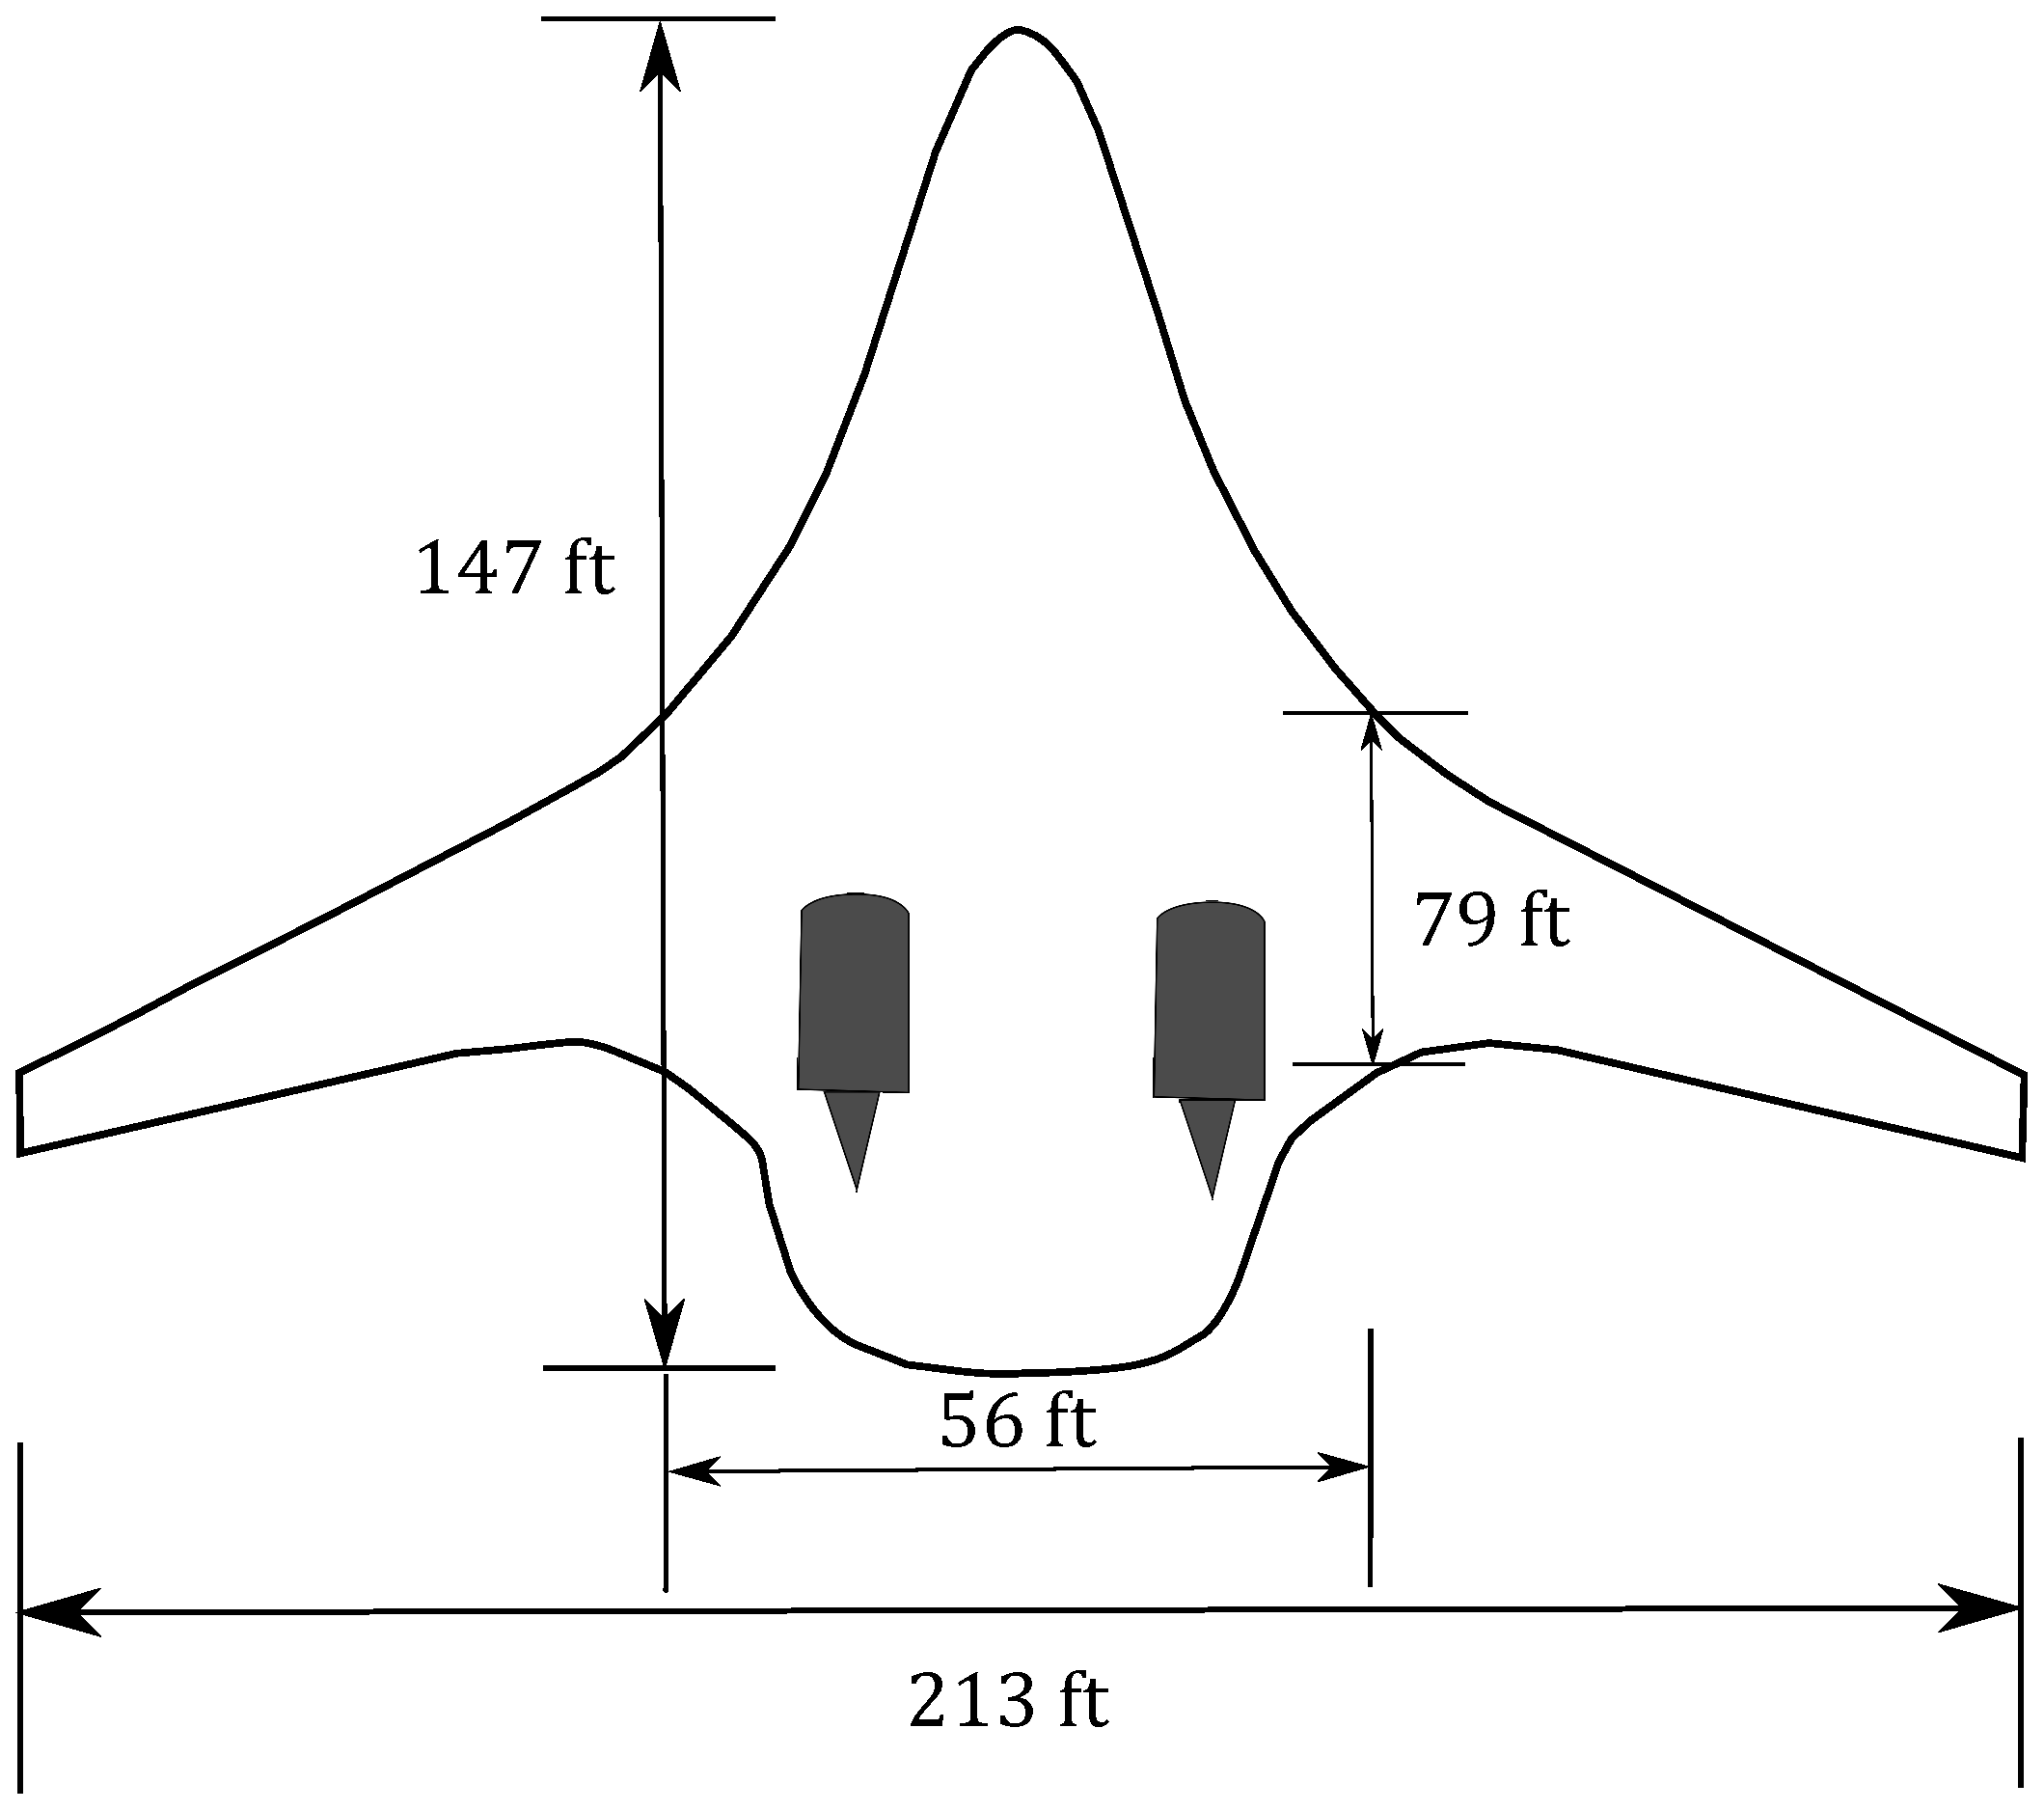
\includegraphics[scale = 0.3]{HWB_Dimensions.eps}
					\captionof{figure}{HWB baseline key design dimensions.}
					\label{Baseline_Design_Table}
				\end{figure}
				

												
			\subsubsection{Available Vehicle Boundary Layer}
			
			
	\section{Baseline Engine}
	\section{BLI Modeling}
		\subsection{Airframe Model}
		\subsection{Power Balance and Drag Book-keeping}
		\subsection{Inlet Model}
		\subsection{Fan Model}
			\subsubsection{General Model Architecture and Algorithm}
			
	\section{Experiment 1 Results}
	
	\subsection{Flight Condition Variation}
	
	\subsubsection{Design Mach Number}
	
	\subsubsection{Design AoA Impact}
	
	\subsection{BLI Design Space Variation}
	
	\subsubsection{Influence of Inlet Aperture Shape}
	
	\subsubsection{Influence of Engine Number}
	
	\subsection{Off-Design Variation}
	
	\subsubsection{Mass Flow Variation}
	
	\subsubsection{Influence of the Pre-entry zone}
	
	\subsubsection{Influence of Flight Condition}
	
	\subsubsection{Impact On MDP Sizing}
	
	\section{Stall Margin Test Experimental Setup}
	
	\subsection{Stall Margin Criteria and Allowables}
	
	\section{Experiment 2 Results}
	
	\section{Summary and Conclusions}